\section{$k$-Nearest Neighbors}

\subsection{Why?} % (fold) \label{sub:why_}

% subsection why_ (end)
The main purpose of implementing nearest neighbor, is to find similar weather
periods in the history and possibly find patterns in the climate. This is useful
in terms of understanding the climate and to forecast specific events. 

As an example, for regions here in Switzerland, it could be useful in terms of avalanche
danger. If most of the nearest neighbors of the current winter so far, led to
many and massive avalanches, it is reason to believe that also the current
winter can become a such a winter. By knowing this, it would be possible to take
action before the events occur. The same method can be used to forecast events
like floods or drought. Nearest neighbor is also used to simulate weather. You pick
an initial start state, compute it's $k$ nearest neighbors. From the set of 
successive states for all the neighbors, you pick one random and set that one as
the weather for the next period. This technique has been used with great success
and has given better results than other ways of simulating weather. 

%It can also be used to find patterns in the climate such as cycles and periodic
%structures. 

%TODO: Rewrite to better language

\subsection{Implementation} % (fold) \label{sub:implementation}

The k-nearest neighbor is a fairly simple algorithm. You choose a metric,
calculate the distance from the reference node to all the other's, and pick the
$k$ nearest neighbors. This has been done more or less straight forward.

In this case a node is a period of time. We fixed the period to one month, such
that you can pick one month for a specific year, and then find the most similar
months for the other years. Often climate data is summarized by month, so this
makes it easy to find data to compare with and verify results.

Next question is to determine how many intervals the period of time should be
divided into. Should we compare averages for an hour, a day, a week, or just one
value for the whole month? For a small region (a few stations) and a short
period of time (a day), then comparing hour by hour could make sense and give
good results. But for a large region (thousands of stations) and for a longer
period (a month), this will mostly just return noise. Here, the method is
implemented with a period option so one can choose how many periods a month
should be divided into. With only one period selected, only the average value
for the whole month is used when calculating the distance to other months.

In mathematical terms, the final expression for the distance between two months
$k$ and $l$, divided into periods $p$, is given by
\begin{equation}
	\label{eq:NN}
	D_{k,l,p} = \frac{1}{n}\sum_{i=1}^{n}{\frac{1}{p}\sum_{j=1}^{p}{
		\sqrt{
			(T_{k,i,j} - T_{l,i,j})^2 + 
			(P_{k,i,j} - P_{l,i,j})^2
		}}},
\end{equation}
where $T_{k,i,j}$ is the average temperature for month $k$ at station $i$ in 
period $j$, $P$ is similar for precipitation and $n$ is the number of stations
that has records for both months $k$ and $l$. Figure (\ref{fig:NNmapReduce}) shows
how this is implemented on Hadoop.

\begin{figure}[tb]
 	\begin{center}
 		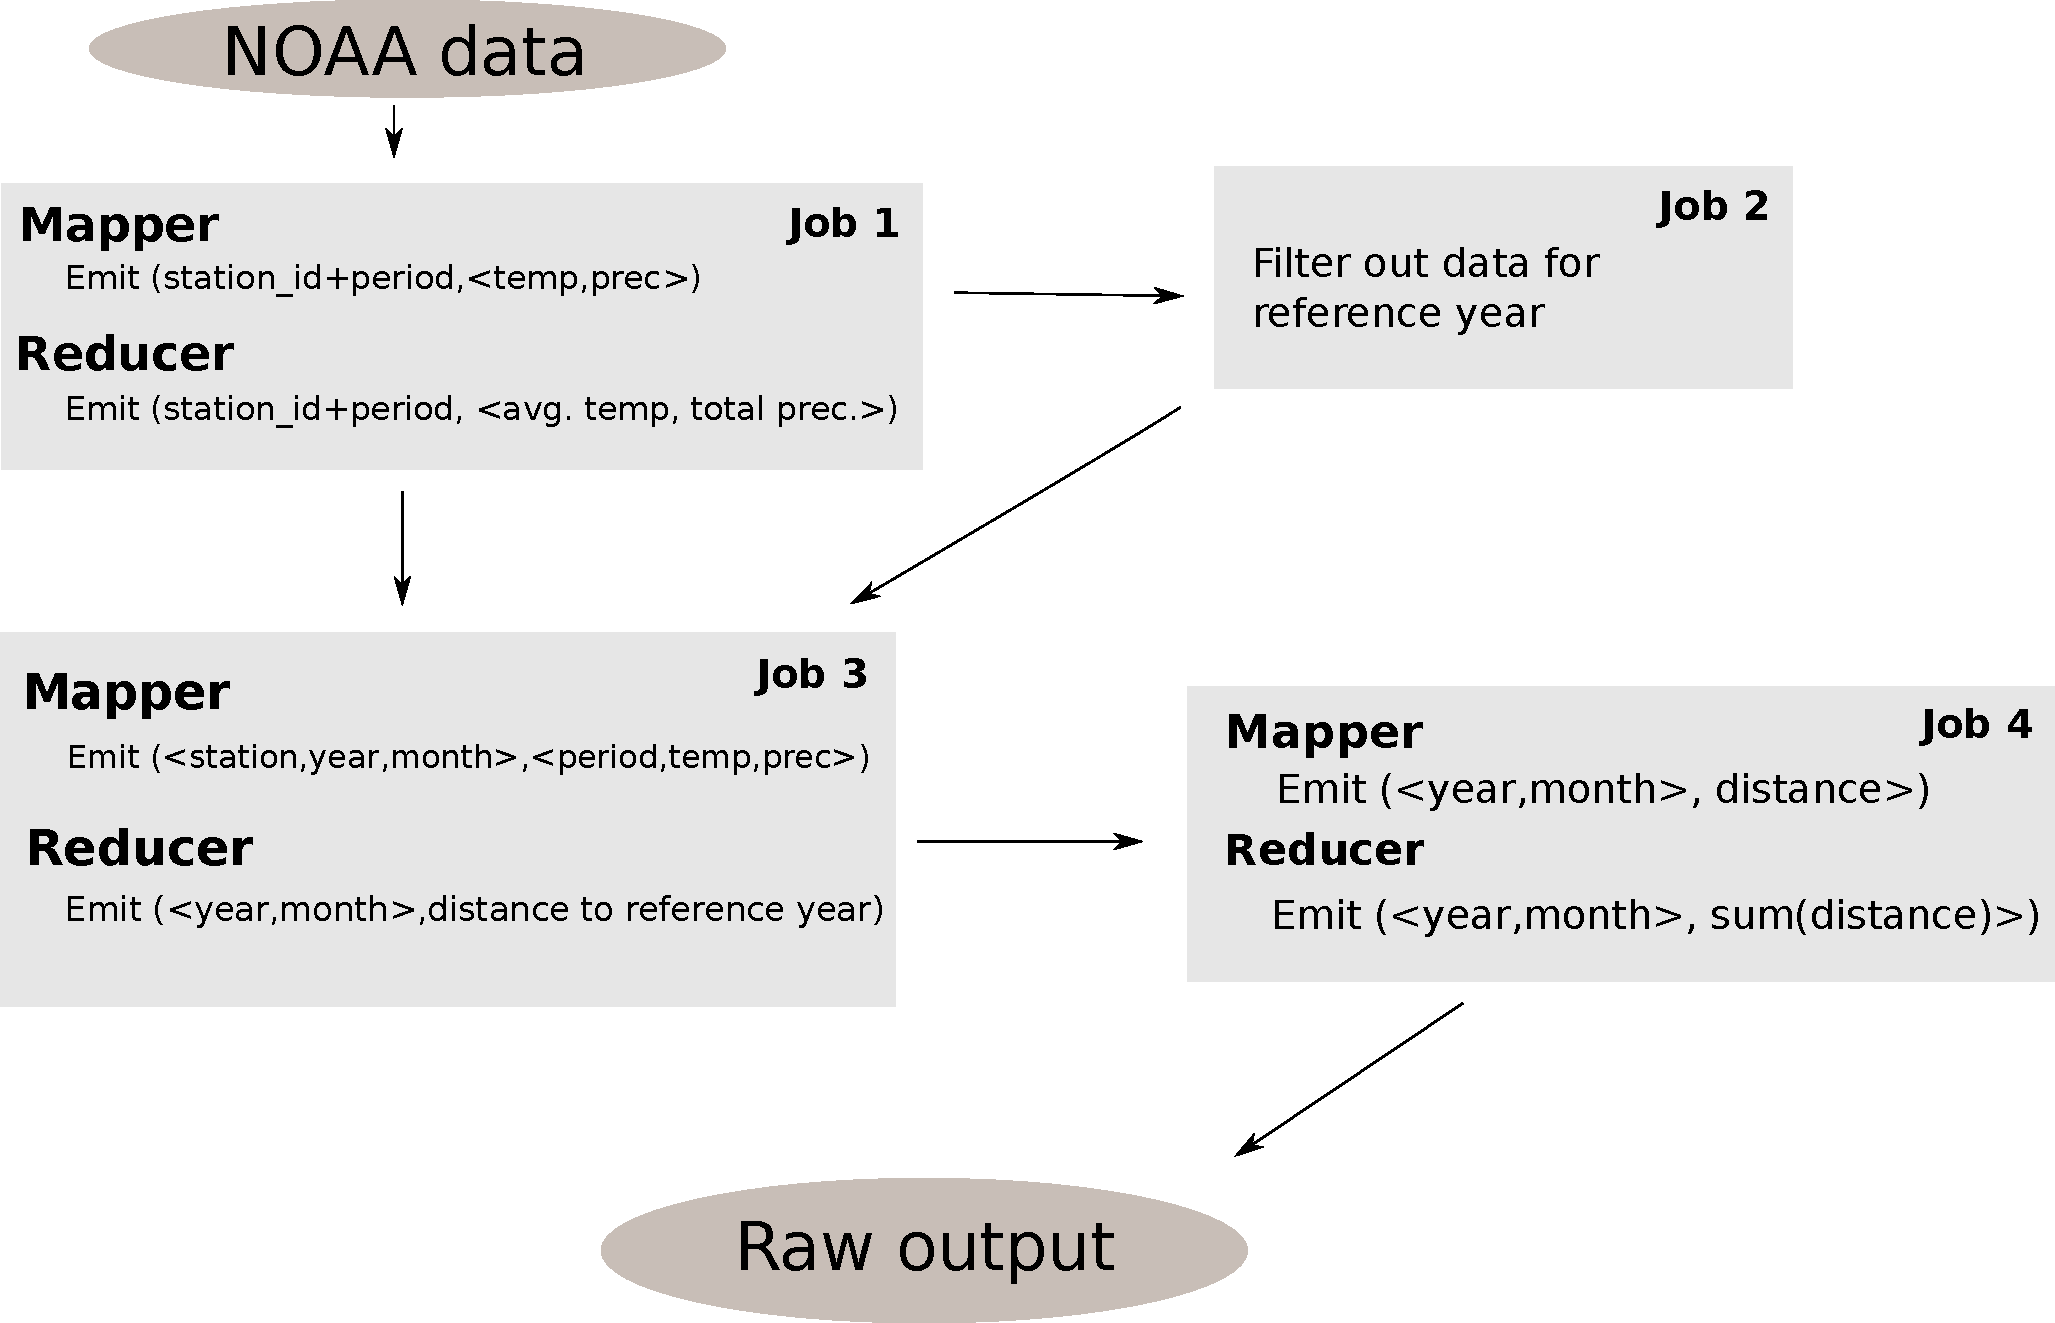
\includegraphics[width=12cm]{figures/NNmapReduce.pdf}
 	\end{center}
 	\caption{Implementation of nearest neighbors in map reduce.}
 	\label{fig:NNmapReduce}
 \end{figure} 

To get good results on the NOAA dataset for USA, which consists of thousands 
of stations, we chose to divide the month into only one period. Thus, equation
(\ref{eq:NN}) reduces to
\begin{equation}
	\label{eq:NN_usa}
	D_{k,l} = \frac{1}{n}\sum_{i=1}^{n}{
	\sqrt{
		(T_{k,i} - T_{l,i})^2 + 
		(P_{k,i} - P_{l,i})^2
	}},
\end{equation}
where $T_{k,i}$ is the average temperature for the whole month $k$ at station $
i$. $P$ is similar for total precipitation. 

% subsection implementation (end)

\subsection{Results} % (fold) \label{sub:results}

We ran the nearest neighbor algorithm on the NOAA dataset for USA. The time period
ranges from 1975 to 2013. In general, and as expected, one can see a strong correlation 
between successive years. It's quite often that the closest neighbor is the year before
or after, at least close in time. So if you want to guess how the weather will be for a
specific month, your best bet would be as it was last year for that month. 

Table (\ref{tab:NN_jul2012}) shows the nearest neighbors for July 2012. Both 2012, 2011 and
2010 were among the warmest July's in US history. They were also very dry in the western parts and
very wet in the eastern parts. 

\begin{table}[ht]
\centering
\caption{Nearest neighbors for July 2012}
\label{tab:NN_jul2012}
\vspace{0.5cm}
\begin{tabular}{rl}
  \hline
  Year & Distance \\ 
  \hline
  2011 & 0.4985 \\ 
  2010 & 0.5299 \\ 
  2008 & 0.5916 \\ 
  1982 & 0.6027 \\ 
  2006 & 0.6027 \\ 
  \hline
\end{tabular}
\end{table}

The graph in figure (\ref{fig:NNgraph}) is one way to visualize the result. Each year is a node, and each
of the nodes is connected to it's two closest neighbors with an edge. The graph shows
how similar years cluster together. There is no axes on the graph, so one needs additional
information to check how the weather was for the specific cluster's of nodes. 

\begin{figure}[tb]
 	\begin{center}
 		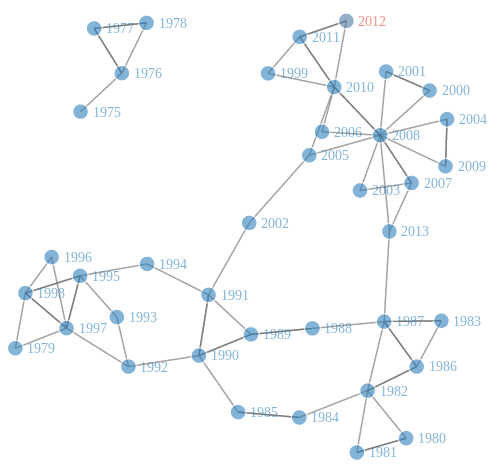
\includegraphics[width=7cm]{figures/NNgraph.png}
 	\end{center}
 	\caption{$k$-nearest neighbors for July visualized with $k = 2$}
 	\label{fig:NNgraph}
 \end{figure} 

%  results (end)
